\documentclass[11pt]{book}
\usepackage[utf8]{inputenc}	% Para caracteres en español

\usepackage[left=2.75cm,right=2.75cm,top=2cm,bottom=3cm]{geometry}
\usepackage{style}
\thispagestyle{fancy}

\author{Arthur Herbette \\
Prof. Michael Gastpar}

\begin{document}
\setcounter{section}{8}
\title{AICC II}
\maketitle
\thispagestyle{empty}
\tableofcontents
\thispagestyle{empty}
\listoflectures

\chapter{Introduction}
\section{About this course}
In this course, there will be three main topics that will be studied:
\begin{itemize}
    \item Communication
    \item Information and Data science
    \item Cryptography, Secrecy, Privacy
\end{itemize}

\section{Cours Grading}
    \begin{itemize}
        \item 90\% Final exam during exam period
        \item 10 \% Quizzes (online on Moodle)
        \begin{itemize}
            \item There will be $6$ quizzes. BO5
            \item On the quizzes, you can update your answer as many times as you want before the deadline
        \end{itemize}
        \item Quizzes are highly coorelated with homework.
    \end{itemize}
\subsection{How to be efficient and do well in this course}
Before class:
\begin{itemize}
    \item Browse through the slides to know what to expect
    \item review the background material as needed
\end{itemize}
After class:
\begin{itemize}
    \item read the notes: they are the reference
    \item do the review questions
\end{itemize}
Before the exercice session
\begin{itemize}
    \item are you up to date with the theory?
    \item Solve what you can ahead of time and finish during the exercice session
    \item write down \textbf{your} solution
\end{itemize}
\lecture{1}{2025-02-18}{Discrete Probability}{}
\section{Initial case: Finite $\Omega$: set of all possiblie outcomes}
\begin{definition}
\textbf{Sample space $\Omega$} is the set of all possible outcomes
\end{definition}
\begin{definition}
    \textbf{Event} $E$: a subset of $\Omega$. Since the outcomes are equally likely: 
    \[p(E) = \frac{|E|}{|\Omega|}\]
\end{definition}
\section{Conditional Probability}
\begin{parag}{Conditional probability}
    \begin{definition}
        The \textbf{conditional probability} $p(E|F)$ is the probability that $E$ occurs, given that $F$ has occured (hence assuming that $|F| \neq 0$) : 
        \[p(E|F) = \frac{|E \cap F|}{|F|}\]
    \end{definition}
\end{parag}
\begin{parag}{Independent Events}
    Event $E$ and $F$ are called \textbf{independent} if $p(E|F) = p(E)$
    \begin{subparag}{Personal remark}
        \begin{framedremark}
            this means that even if we know that $F$ has occured the probability of $E$ is still the same.
        \end{framedremark}
    \end{subparag}
\end{parag}
\begin{parag}{General Case: Finite $\Omega$, arbitary $p(\omega)$}
    Having equally likely outcomes is pretty rare in real life, juste take two dices and do the sum of the result and you will se that all the possible outcome doesn't have the same probability. In order to express those types of distribution we use the probability mass function:
    \begin{definition}
        \textbf{Sample space} $\Omega$: set of all possiblie outcomes
        \\
        \textbf{Probability distribution (probability mass function) $p$} : 
        \\
        A function $p : \Omega \to 1$ such that: 
        \[\sum_{\omega \in \Omega} p(\omega) = 1\]
    \end{definition}
    If we sum up all the probablity it gives us $1$.
     \begin{subparag}{muss function to a subset}
         Given $E \subset \Omega$ we can define the domain of the probability mass function $p$ is extended to the power set of $\Omega$ : 
         \[p(E) = \sum_{\omega \in E} p(\omega)\]
     \end{subparag}
\end{parag}
\section{Conditional probability and Independent Events}
\begin{parag}{General form}
    The general form for the conditional probability is:
    \[p(E|F) = \frac{p(E \cap F)}{p(F)}\]
    for $F$ such that $p(F) \neq 0$
\end{parag}
\begin{parag}{Independet events}
    As before $E$ and $F$ are called independent if $p(E|F) = p(E)$, Equivalently, $E$ and $F$ are independent iff $p(E \cap F) = p(E)p(F)$.
\end{parag}
\begin{parag}{Disjoin event}
    if $E_1$ and $E_2$ are disjoint event then:
    \[p(E_1 \cup E_2) = p(E_1) + p(E_2)\]
\end{parag}
\begin{parag}{Law of total probability}
    For any $F \subseteq \Omega$ and its complement $F^c$,
    \[p(E) = p(E|F)p(F) + p(E|F^c)p(F^c)\]
    which sounds very intuitive because by definition $F$ and $F^c$ are disjoint.
    \begin{subparag}{Generally}
    \begin{theoreme}
        If $\Omega$ is the union of disjoint event $F_1, F_2, \dots, F_n$ then:
        \[p(E) = p(E|F_1)p(F_2) + p(E|F_2)p(F_2) + \cdots + p(E|F_n)p(F_n)\]
    \end{theoreme}
\end{subparag}
\begin{subparag}{Proof}
    We prove the law of total probability for $\Omega = F \cup F^c$ (the general case follows straighforwardly)
    \begin{align*}
        p(E) &= p((\underbrace{E \cap F) \cup(E \cap F^c)}_{\text{union of disjoint sets}})\\
        &= p(E \cap F) + p(E \cap F^c) \\
        &= \frac{p(E \cap F)}{p(F)}p(F) + \frac{p(E \cap F^c)}{p(F^c)}p(F^c) \\
        &= p(E|F)p(F) + p(E|F^c)p(F^c)
    \end{align*}
\end{subparag}
\end{parag}
\begin{parag}{Bays' Rule}
    \begin{theoreme}
        \[p(F|E) = \frac{p(E|F)p(F)}{p(E)}\]
    \end{theoreme}
    \begin{subparag}{Proof}
        We use the definition of conditional probability to write $p(E \cap F)$ two ways and solve for $p(F|E)$:
        \[p(F|E)p(E) = p(E \cap F) = p(E|F)p(F)\]
    \end{subparag}
\end{parag}

\section{Random variable}
\begin{parag}{Random variable}
    \begin{definition}
        A Random variable is a function $X$ such as $X : \Omega \to \mathbb{R}$
    \end{definition}
\end{parag}
\begin{parag}{Probability distribution}
    $p_x$, $p_x(X = x)$ or $p_x(x)$ is the probability that $X = x$, i.e, the probability of the event
    \[E = \{\omega \in \Omega: X(\omega) = x\}\]
    Hence,
    \[p_x(x) = \sum_{w \in E}p(\omega)\]
    \begin{subparag}{Example}
        You rolle a dice.
        \\
        if the outcome is $6$, you receive $10$CHF. Otherwise, you pay $1$ CHF.
        \[\Omega = \{1, 2, 3, 4, 5,6\}\]
        \[\text{For each }\omega,p(\omega) = \frac{1}{6}\]
        Then define:
        \[X(\omega) = \begin{cases}
            10, \; \; \omega = 6 \\
            -1, \; \; \omega \in \{1, 2, 3, 4, 5\}
        \end{cases}\]
        Hence, we have
        \[p_x(X) = \begin{cases}
            \frac{1}{6}, \; \; x = 10 \\
            \frac{5}{6}, \; \; x = -1
        \end{cases}\]
    \end{subparag}
\end{parag}
\subsection{Two random variables}
\begin{parag}{Two random variables}
    \begin{definition}
        Let $X: \Omega \to \mathbb{R}$ and $Y: \Omega \to \mathbb{R}$ be two random variables.
        \\
        The probability of the event $E_{x, y} = \{w \in \Omega: X(\omega) = x$ and $Y(\omega) = y\}$ is:
        \[p_{x, y}(x, y) = \sum_{w \in E_{x, y}} p(\omega)\]
    \end{definition}
    \begin{itemize}
        \item $p_x$ is called \important{marginal distribution} (of $p_{x, y}(x, y)$ with respect to $x$)
        \item $p_y$ can be computed similarly
    \end{itemize}
\end{parag}
\section{Expected Value}
\begin{parag}{Expected value}
    \begin{definition}
        The expected value $\mathbb{E}[X]$ of a random variable $X:  \Omega \to \mathbb{R}$ is : 
        \[\E[X] = \sum_\omega{X(\omega)p(\omega)}\]
        \[= \sum_x xp_x(x)\]
    \end{definition}
\end{parag}
\begin{parag}{linearity}
    Expectation is a linear operation in the folowwing sence:
    \\
    Let $X_1, X_2, \dots, X_n$ be random variables and $\alpha_1, \alpha_2, \dots, \alpha_n$ be scalars. Then:
    \[\E \left[\sum_{i=1}^n X_i\alpha_i\right] = \sum_{i=1}^n\alpha\E [X_i]\]
\end{parag}
\begin{parag}{Random variable and independecy}
    Two random variable $X$ and $Y$ are independent if and only if, for all realizations $x$ and $y$:
    \[p(\{X = x\} \cap \{Y = y\}) = p(\{X = x\}) p(\{Y = y\})\]
    Or, more concisely, iff
    \[p_{x, y}(x, y) = p_x(x)p_y(y)\]
\end{parag}
\begin{parag}{Generalization}
    \begin{theoreme}
        Given $n$ random variables, $X_1, \dots, X_n$ are independent if and only if:
        \[p_{x_1, \dots, x_n}(x_1, \dots, x_n) = \prod_{i = 1}^n p_{x_i}(x_i) \]
    \end{theoreme}
\end{parag}
\begin{resume}
\begin{itemize}
    \item Random Variable
    \item Probability distribution
    \begin{itemize}
        \item Joint distribution of multiple variables
        \item Marginal distribution
        \item Conditional distribution
    \end{itemize}
    \item Independence
\end{itemize}    
\end{resume}
\lecture{2}{2025-02-19}{Source and entropy}{}

\begin{parag}{Expected value and operation}
    The addition works well with Expectation such that
    \[\E[X + Y] = \E[x] + \E[Y]\]
    However, the product doesn't work well, \\
    \[\E[XY] = \E[X]\E[Y]\]
    \important{if and only if} $X$ and $Y$ are independent random variables.
    
\end{parag}
\section{Entropy}
\begin{parag}{Introduction}
    We communicate be revealing the value of sequence of variables that we call (\textbf{Symbols}), \textbf{Information}
    \\
    In modern language, Hartley was saying that the value of a symbole provides information if and only if the symbol is a \textbf{random variable}.
    \\
    How much information is carried by a symbol such as $S$?
    \begin{itemize}
        \item Suppose that  $S \in \mathcal{A}$ is a symbol that can take $|\mathcal{A}|$ possible values
        \item The amount of information conveyed by $n$ such symbol should be $n$ times the informations conveyed
        \item there are $|\mathcal{A}|^n$ possible values for $n$ symbols
        \item This suggests that $\log|\mathcal{A}|^n = n\log |\mathcal{A|}$ is the appropriate mesure for information
    \end{itemize}
    However, this approach doesn't works:
    \begin{subparag}{Example}
        Imagine having a town where there are $360$ days and $5$ rainy days, this leads to have only to possibilities, $|\mathcal{A}| = 2$ which make the quantity of information $\log_2 2 = 1$ bits. Which intiutively sounds kind of false, the forecast doesn't give us that information knowing that it is sunny $\frac{360}{365}$ \% of the times, it is kind of excpected. 
    \end{subparag}
    An article in 1948 from Shannon fixes the problem by defining \textbf{Entropy}
\end{parag}
\begin{parag}{Definition}
    the \textbf{uncertainty} or \textbf{entropy} $H(S)$
    associated to a discrete random variable $S$:
    \begin{definition}
        \[H_b(S) = - \sum_{S \in supp(p_s)}p_s(s)\log_bp_s(s)\]
        Where sup$p(s) = \{s : p_s(s) > 0\}$.
    \end{definition}
\end{parag}
\begin{parag}{Few comments}
    \[H_b(S) = - \sum_{S \in supp(p_s)}p_s(s)\log_bp_s(s)\]
    \begin{itemize}
        \item The condition $S \in supp(p_s)$ is needed because $\log_bp_s(s)$ is not define when $p_s(s) = 0$ this convention allows us to use the notation : 
        \[H_b(S) = - \sum_{s \in \mathcal{A}}p_s(\log_bp_s(s))\]
        \item The choice of $b$ determines the unit, $b= 2$ is the \important{bit}
    \end{itemize}
    We also can see this as an "\textit{average}" of $-\log_b p_s(S)$ which is:
    \[H(S) = \E [-\log_bp_s(S)]\]
\end{parag}

\begin{parag}{Example}
    A sequence of $4$ decimal digits, $s_1, s_2, s_3, s_4$ representing the number to open Anne's lock can be senn as the output of a source $S_1, S_2, S_3, S_4$ with $S_i = \{0, \dots, 9\}$.
    \\
    If Anne picks all digits at randm and indepedently, the all outcomes are equally likely:
    \[p_{S_1, S_2, S_3, S_4}(S_1, S_2, S_3, S_4) = \frac{1}{10^4}\]
    If we search the entropy of this we get:
    \[H_2(S) = \log_2|\mathcal{A}| = \log_2 10^4 \approx 13.3 \; bits\]
\end{parag}

\subsection{Information-Theory Inequality}
\begin{parag}{Lemma (IT-Inequality)}
    \begin{lemme}
        For a positive real number $r$, 
        \[\log_b r \leq (r-1)\log_b(e)\]
        with equality if and only if $r = 1$
    \end{lemme}
    This proof juste using the deriative
    
\end{parag}
\begin{parag}{Entropy Bounds}
    \begin{theoreme}
        The entropy of a discrete  random variable $S \in \mathcal{A}$ satisfies:
        \[0 \leq H_b(S) \leq \log_b|\mathcal{A|}\]
        With equality on the left if and only if  $p_s(S) = 1$ and on the right if and only if $p_s(S) = \frac{1}{|\mathcal{A}|}$ for all  $s$.
    \end{theoreme}
\end{parag}
\subsection{Random variables and Entropy}
\begin{parag}{$n$ random variable}
the formula for entropy can be expanded to any number of random variables. If $X$ and $Y$ are two discrete random variables, with (joint) probability distribution $p_{x, y}$ then:
\[H(X, Y) = -\sum_{(x, y) \in X \times Y} p_{x, y}(x, y)\log p_{x, y}(x, y)\]
\end{parag}
\begin{parag}{1.4 of textbooks}
    \begin{theoreme}
        Let $S_1, \dots, S_n$ be discrete random variables. Then
        \[H(S_1, S_2, \dots, S_n) \leq H(S_1) + H(S_2) + \cdots + H(S_n)\]
        With equality if and only if $S_1, \dots, S_n$ are indepedent.
    \end{theoreme}
\end{parag}











\begin{parag}{Ex hat party 1950}
    \begin{itemize}
        \item $n$ men, all have the same hat
        \item they throw hats in a corner
        \item leaving, they randomly take a hat
    \end{itemize}
    \begin{subparag}{Solution}
        Let $R_i = \begin{cases}
            1, \text{ if person } i \text{ leaves with their own hat} \\
            0, \text{ otherwise}
        \end{cases}$\\
    There we search the Expected value here:
    \begin{align*} 
        \mathbb{E}\left[R_1 + R_2 + \cdots + R_n\right] &= \mathbb{E}\left[R_1\right] + \mathbb{E}\left[R_2\right] + \cdots + \mathbb{E}\left[R_n\right]\\
                                                        &= \frac{1}{n} + \frac{1}{n} + \cdots + \frac{1}{n}\\
                                                        &= 1
    \end{align*}

   Then we know that, on average, only one person get the right hat.
    \end{subparag}

\end{parag}
\lecture{3}{2025-02-25}{suite}{}
\begin{parag}{Entropy}
    \begin{equation} H_2(S) =\sum_i p(s)\log \frac{1}{2p(s)} \end{equation}
    \begin{equation} = \frac{1}{8}\log_2 \frac{8}{2} + \frac{1}{8} \log_2 8 \end{equation}
   
    
    \begin{equation} \approx \frac{1}{8} + \frac{1}{8} \cdot 3 \end{equation}
    
  \begin{subparag}{personal remark}
      We can see it as an average of "surprise".
      \\
      Where the average is the randomness. ($\approx 0.55$)
  \end{subparag}  
\end{parag}

\subsection{Entropy bounds}

\begin{parag}{Bound}
    \begin{align*}
        0 \leq H_b(S) \leq \log_b \mathcal{A}
    \end{align*}
    
\end{parag}

    \section{Source Coding Purpose}
    Source coding is often seen as a way to compress the source.
    \\
    More generally, the foal of source coding is to efficiently describe how much information there is to a \textit{file}
    
 \subsection{Setup}
 \begin{parag}{Setup}
     The \textbf{encoder} is specified by:
     : \
\begin{itemize}
    \item the input alphabet$ \mathcal{A}$ (the same as the source alphabet)
    \item the output alphabet $\mathcal{D} $(typically  $ \mathcal{D} = \{0, 1\}$);
    \item the codebook $\mathcal{C} $ Which consists of finite sequences over $ \mathcal{D}$;
    \item By the one to one encoding map $ \Gamma : \mathcal{A}^k \to \mathcal{C}$ where $k$ is a positive integer.
\end{itemize}
For now, $k = 1$.


 \end{parag}
 
 \begin{parag}{Example}
     For each code, the encoding map $ \Gamma$ is specified in the following table:
     \begin{center}
         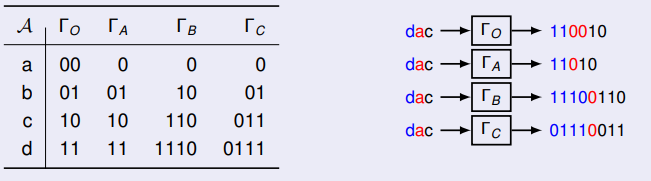
\includegraphics[scale=0.8]{12025-06-02.png}
     \end{center}
     
 
 \end{parag}
\begin{parag}{Decodability}
    We want to avoir the following problem (encoding map $\Gamma_A$ )
    \begin{align*}
        cbaad \to 100010011 \begin{cases} \to cbaad \\ \to cacad
    \end{align*}

    \begin{definition}
        The code is uniquely decodable if every concatenation of codewords has a unique parsing into a sequence of codewords.
    \end{definition}
    
    Recall that the encoding function $\Gamma$ is one to one by assumption
    \begin{subparag}{Example}
        Code $C$ or $B$ are uniquely decodable : 
        (A mettre une image 106)
    \end{subparag}
\end{parag}
 
\begin{parag}{Prefix Free codes}
    \begin{definition}
        If no codeword is a prefix of another codeword, the code is said to be prefix free.
    \end{definition}
   \begin{subparag}{Example}
        The codeword \important{01} is a prefix of \important{01}1. \\

       
   \end{subparag}
   \begin{itemize}
       \item A prefix free code is always uniquely decodable
       \item A uniquely decodable code is \important{not necessarily} prefix free
   \end{itemize}
   \begin{subparag}{A prefix code }
       A prefix free code is also called instantaneous code : 
       \begin{itemize}
           \item Think of phone numbers
           \item Think about streaming: instantaneous codes minimize the decoding delay (for given codeword length)
       \end{itemize}
   \end{subparag}
\end{parag}
 
\begin{parag}{Code for one random variable}
    We start by considering codes that encode \important{one single random variable} $ S \in \mathcal{A}$.
    \\
    To encode a sequence $S_1, S_2, \dots $ of random variables, we encode one random variable at a time.
\end{parag}

\begin{parag}{Complete tree of a code}
    Slide 113 screen.
\end{parag}
\begin{parag}{Binary tree}
    \begin{itemize}
        \item There is a \improtant{root} (the beginning)
        \item A vertex (another node)
        \item A \important{leaf} is the last vertex
        \item Which is like a (arbre généalogique)
    \end{itemize}
\end{parag}
\begin{parag}{Ternary Tree}
    The same as a binary tree but with three children.
\end{parag}

\begin{parag}{With/Without prefix}
slide 115.
\end{parag}

\begin{parag}{Decoding tree}
    \begin{itemize}
        \item Obtained from the complete tree by keeping only branches that form a codeword
        \item Useful to visualize the decoding process
    \end{itemize}
    Slide 116
\end{parag}

\subsection{Codeword length}
    \begin{itemize}
        \item The codeword length is defined the obvious way:
        \item Example: 
            \begin{center}
            \begin{tabular}{|c|c|c|}
            \hline
                $ \mathcal{A}$ & $ \Gamma_B$ & codeword lengths \\
            \hline
            \hline
                $a$ & $0$ & $1$ \\
            \hline
                $b$ & $10$ & $2$ \\ 
            \hline
                $c$ & 110 & 3 \\
            \hline
                $d$ & 1110 & 4
            \hline
             \end{tabular}
            \end{center}
         \item We would like the average codeword length to be as small as possible.
    \end{itemize}
\subsection{Kraft McMillan}
\begin{parag}{Part 1. Necessary condition for the code to be uniquely decodable}
    \begin{theoreme}
        If a $D$-ary code is uniquely decodable then its codeword length $i_1, \dots, i_M$ satisfy
        \begin{align*}
            D^{-l_1} + \cdots  + D^{-l_M} \leq i 
        \end{align*}
        Kraft's inequality
    \end{theoreme}
  \begin{subparag}{Example}
        For code $O$ we have : 
        \begin{align*}
            2^{-2} + 2^{-2} + 2^{-2} + 2^{-2} = 1
        \end{align*}
        
  \end{subparag}

\end{parag}

\begin{parag}{contrapositive of Kraft McMillan part 1}
\begin{subparag}{Example A}
    For code $A$ we have $2^{-1} + 2^{-2} + 2^{-2} + 2^{-2} = 1.25 > 1$
    .
    \\
    KRaft-McMillan's inequality is not fulfilled. \\
    There exists no uniquely decodable code with those codeword lengths.
\end{subparag}    
\end{parag}

\begin{parag}{Proof of K-MM Part I}
    We prove a slightly weaker result, namely that the codeword lengths of prefix free codes satisfy K-MM inequality.
    \\
    Let $L = \text{max}_i l_i$ be the complete tree's depth. 
    \begin{itemize}
    \item There are $D^L$ terminal leaves
        \item There are $D^{L-l_i}$
        \item No two codewords share a terminal leaf (The code is prefix free)
        \item Hence $D^{L-l_i} + D^{L-l_2} + \cdots  + D^{L-l_m} \leq D^L$
    \end{itemize}
    After dividing both sides by $D^L$ we obtain Kraft's inequality:
    \begin{align*}
        D^{-l_1} +  D^{-l_2} + \cdots  + D^{-l_M} \leq 1
   \end{align*}
    \begin{subparag}{Exercice}
        What is the \important{converse} of Kraft McMillan part 1?
        \\
        The \important{Converse} of Kraft McMillan part 1 is not true (Consider e.g. two codewords: 01 and 0101)
        \\
        However, the following statement is almost as good : 
        \begin{theoreme}
            If the positive integer $I_1, \dots, I_M$ satisfy Kraft's inequality for some positive integer $D$,then there exists a D-ary \important{prefix free code} (hence uniquely decodable) that has codewords
        \end{theoreme}
        
        This says that if the inequality is true, then we \important{can} find D \text{ such that } there exists a binary prefix which makes it decodable \important{and} prefix free!
    \end{subparag}
\end{parag}

\subsection{Important Consequence of Kraft McMillan}
\begin{parag}{Part I}
\begin{theoreme}
    If a \important{D-ary code is uniquely decodable}, then its codeword length $I_1, \dots I_M$ satisfy Kraft's inequality : 
    \begin{align*}
        D^{-l_1} + \cdots  + D^{-l_M} \leq 1
    \end{align*}
    
\end{theoreme}

\end{parag}
\begin{parag}{Part II}
    \begin{theoreme}
        If the positive integer $l_1, \dots, l_M$ satisfy Kraft's inequality for some positive integer $D$, then there exists a D-ary \important{prefix free code} that has those codeword lengths.
    \end{theoreme}
   The Kraft McMillan theorem implies that any uniquely decodable code can be substituted by a prefix free code of the same codeword lengths. 

\end{parag}

\begin{parag}{Prefix free codes}
    Our focus will be on prefix free codes. Reasons:
    \begin{itemize}
        \item No loss of optimality: codewords can be as short as for any uniquely decodable code;
        \item a prefix free codeword is recognized as soon as its last digit is seen:
            \begin{itemize}
                \item important, e.g. a phone number;
                \item advantageous to limit the decoding delay in, say streaming
            \end{itemize}
    \end{itemize}
\end{parag}

\begin{parag}{Average Codeword length}
    \begin{itemize}
        \item The typical use of a code is to encode a sequence of random variables
            \item
    \end{itemize}
    \begin{subparag}{Example}
        \begin{align*}
            \mathcal{A} = \{a, b, c, d\} \; \; D = 2
        \end{align*}
        Blackboard with table
        \begin{tabular}{cccc}
            $s \in \mathcal{A} $ & $ \Gamma (s)$ & $l(s)$ & $p(s)$ \\
            \hline \\ \hline
            \\
            $a$ & $ 0$ & 1 & 0.05 \\
            \hline 
            b & 10 & 2 & 0.05 \\
            c & 110 & 3 & 0.1 \\
            d & 1111 & 4 & 0.8
        \end{tabular}

        \begin{align*}
            \mathcal{E} [ \text{length} ] = 0.05 + 1 + 0.05 \cdot 2
        \end{align*}
        
             
        

    \end{subparag}
    \begin{definition}
        Let $l( \Gamma (s))$ be the length of the codeword assiociated to $s \in \mathcal{A}$ The average codeword length is:
        \begin{align*}
            L(S, R) = \sum_i p_s(s) i ( \Gamma (s)) 
        \end{align*}
        
    \end{definition}
    
        \begin{subparag}{Units}
            The unit of $L(S, \Gamma ) $ are \important{code symbols}
            \\
            When $D = 2$, the unit of $L(S, \Gamma )$ are bits.
        \end{subparag}
\end{parag}


\begin{parag}{Average codeword length: Lower Bound}
    \begin{theoreme}
        Let $ \Gamma : \mathcal{A} \to \mathcal{C}$ be the encoding map of a D-ary code for the random variable $S \in \mathcal{A}$ .\\
        If the code is uniquely decodable, then the average codeword length is lower bounded by the entropy of $S$ namely:
        \begin{align*} 
            H_D\left(S\right) \leq L\left(S, \Gamma\right)
        \end{align*}
        With equality if and only if for all $s \in \mathcal{A}$, $p_S\left(S\right) = D^{-l\left(\Gamma\left(s\right)\right)}$. An equivalent condition is:
        \begin{align*} 
            l\left(\Gamma\left(s\right)\right) =  \log_D \frac{1}{P_S\left(S\right)}
        \end{align*}
    \end{theoreme}
    \begin{subparag}{Proof}
        We want to prove that:
        \begin{align*}
            H(s) - \sum_s p(s)l(s) \\
            &= - \sum_s p(s) \log p(s) - \sum_s p(s)l(s) \\
            &= - \sum_s p(s)\log p(s) - \sum_s p(s) \log 2^{l(s)} \\
            &= -\sum_s p(s) \log (p(s) \cdot 2^{l(s)}) \leq \dots
        \end{align*}
        Therefore:
        \begin{align*}
            &= \sum_s p(s) \log ( \frac{1}{p(s)}2^{-l(s)}) \\
            &\leq \sum_s p(s) \left( \frac{1}{p(s)}2^{-l(s)} -1 \right) \cdot C \\
            &= (\sum_s 2^{-l(s)} - \sum_s p(s)) \cdot C \\
            &\leq 0
        \end{align*}
        
        We know that the left side is less or equal to $1$ because of the Kraft Inequality, therefore it is bounded.
        
    \end{subparag}
\end{parag}




\lecture{4}{2025-02-26}{Continue}{}


\begin{parag}{Key observation}
    The right hand side of:
    \begin{align*}
        L(S, \Gamma) = \sum_{s \in \mathcal{A}} p(s) l ( \Gamma (s))
    \end{align*}
    \begin{align*}
        H_D(S) = \sum_{s \in \mathcal{A}} p(s) \log_D \frac{1}{p_S(s)}
    \end{align*}
    are identical if $l( \Gamma (s))$
    \begin{itemize}
        \item Unfortunately $l( \Gamma (s)) = \log_D \frac{1}{p_S(s)}$ is often not possible (not an integer)
        \item How about choosing
    \end{itemize}
    
    \begin{theoreme}
        \begin{itemize}
            \item For every random variable $S \in \mathcal{A}$
        \end{itemize}
    \end{theoreme}
\end{parag}

\begin{parag}{Theorem}
    
    \begin{theoreme}
        The average codeword length of a D-ary Shannon-Fano code for the random variable $S$ fulfils: 
        \begin{align*}
            H_D(S) \leq L(S, \Gamma_{SF}) < H_D(S) + 1
        \end{align*}
        
    \end{theoreme}
   \begin{subparag}{Proof}
       it suffices to prove the upper bound (we have already proved the lower bound) 
       \\
       First suppose that we could use $l_i = -\log p_i$. The average length would be:
       \begin{align*}
           L(S, \Gamma) = \sum_i p_i l_i = \sum_i p_i (-\log_D p_i) = H_D(S)
       \end{align*}
       Instead we use $l_i = \left\lceil -\log p_i \right \rceil < - \log p_1 + 1 $
       
   \end{subparag} 

\end{parag}


\lecture{5}{2025-03-04}{Conditional Entropy}{}


\begin{parag}{Key Idea}
    Pack multiple symbols into " \textit{supersymbols}"
    \begin{itemize}
        \item $(S_1, S_2, S_3, \dots, S_n)$
        \item Now, apply our Main result to such supersymbols
    \end{itemize}
    \begin{theoreme}
        The average codeword-length of a uniquely decodable code $ \Gamma$ for $S$ must satisfy:
        \begin{align*}
            H_D(S_1, S_2, \dots, S_n) \leq L((S_1, S_2, \dots, S_n), \Gamma)
        \end{align*}
        And there exists a uniquely decodable code $ \Gamma_{SF}$ satisfying:
        \begin{align*}
            L((S_1, S_2, \dots, S_n), \Gamma_{SF}) < H_D(S_1, S_2, \dots, S_n) + 1
        \end{align*}
    \end{theoreme}
\end{parag}

\begin{parag}{Our Next Nugget}
    Understand

    \begin{subparag}{Example}
        Audio recording:
        \begin{itemize}
            \item We can easily anticipate the next image in a video, there
        \end{itemize}
    \end{subparag}

\end{parag}

\begin{parag}{KEy(simple) Independent}
    \begin{definition}
        The source models a seuquence $S_1, S_2, \dots, S_n$ of $n$ coin flips
        \\
        So $S_i \in \mathcal{A} = \{H, T\}$ where $H$ stands for heat, T for tails.
        \\
        $p_{S_i}(H) = p_{S_i}(T) = \frac{1}{2}$ for all $(s_1, S_2, \dots, S_n) \in \mathcal{A}^n$
    \end{definition}

    

\end{parag}

\begin{parag}{Not independent}
    \begin{definition}
        The source models a sequence $S_1, S_2, \dots, S_n$ of weather conditions.
        \\
        So $S_i \in \mathcal{A} = \{S, R\}$, where $S$ stands for sunny and $R$ for rainy\\
        The weather on the first day is uniformly distributed in $ \mathcal{A}$.
        \\
        For all other days, with probability $q = \frac{6}{7}$ the weather is as for the day before
    \end{definition}
    

\end{parag}


 \begin{parag}{Conditional Probability}
     Recall how to determine the conditional probability:
     \begin{align*}
         p_{X\mid Y}(x \mid y) = \frac{p_{X, Y}(x, y)}{p_Y(y)}
     \end{align*}
     It gives the probability of the event $X = x$, given that the event $Y = y$ has occured. \\ it is defined for all $y$ for which $p_Y(y) > 0$
     \begin{subparag}{Remark}
         There is good slide with good schema in slide 176-179
         
     \end{subparag}
 \end{parag}

 \begin{parag}{Conditional Expectation of $X$ given $Y = y$}
     \begin{align*}
         p_{X \mid Y}( \cdot \mid y)
     \end{align*}
     is the probability distribution of the alphabet of $X$, juste like $p_x( \cdot)$
     \begin{definition}
         The conditional expectation of $X$ given $Y = y$ is defined as:
         \begin{align*}
             \mathcal{E}[X \mid Y = y] = \sum_{ x \in \mathcal{X}}
         \end{align*}
         
     \end{definition}
     
     
 
 \end{parag}

 
 \begin{parag}{Conditional Entropy of $X$ given $Y = y$}
     $p_{X \mid Y}( \cdot \mid  y)$ is a probability distribution on the alphabet of $X$, juste like $p_X( \cdot)$ Every probability distribution has an entropy associated to it:
     \begin{itemize}
         \item $p_x( \cdot) \to H(X)$
         \item $p_{ X \mid  Y}( \cdot \mid y) \to H(X \mid Y = y)$
     \end{itemize}
     \begin{definition}
         The conditional entropy of $X$ given $Y = y$ is defined as:
         \begin{align*}
             H_D ( X \mid Y = y) = - \sum_{x \in \mathcal{X}} p_{X \mid Y}(
         \end{align*}
         
     \end{definition}
     \begin{subparag}{Example}
         A faire
         
     \end{subparag}
 
 \end{parag}
 \begin{parag}{Entropy Bounds}

     \begin{theoreme}
         The conditional entropy of a discrete random variable $X\in \mathcal{X}$ conditioned on $Y = y$ satisfies:
         \begin{align*}
             0 \leq H_D(X \mid Y = y) \leq \log_D \mid \mathcal{X} \mid
         \end{align*}
     With equality on the left iff $p_{X \mid Y}(x, y) = 1$ for some $x$, and with equality on the right iff $p_{X \mid Y}(x \mid y) = \frac{1}{\mid \mathcal{X}\mid }$
         
     \end{theoreme}
     The proff is identical to our proof of the basic entropy bounds
 
 \end{parag}
 
 \begin{parag}{Example}
     Question?
     \\
     Do we also have the following entropy bound:
     \begin{align*}
         H_D(X \mid > = y) \overbrace{ \leq}^{???} H_D(X)?
     \end{align*}
     Answer: no.

     \begin{subparag}{Example}
         (Or " \textit{counterexample}" if better), Juste for ease of calculation, let us set $ \delta = 0$ (but this is not necessary for the example to work). Then, we have:
         \begin{align*}
             H_D(X \mid Y = 0) h_D( \epsilon) \text{ and } H_D(X \mid Y= 1) = 0
         \end{align*}
         where $h_d( \cdot)$ is the binary entropy function (with $\log_D( \cdot)$). But we have:
         \begin{align*}
             H_D(X) = h_D( \frac{1 - \epsilon}{2})
         \end{align*}
     \end{subparag}
     \begin{framedremark}
         Conditional entropy can either go up or down (if we give the answer the entropy is $0$)
     \end{framedremark}
 \end{parag}
 \begin{parag}{Conditional Entropy of $X$ given $Y$}
     The most useful and impactful definition is the \textit{average} conditional entropy of $X$ given $Y = y$, averaged over all values of $y$ under the marginal distribution $p_Y(y)$. Formally, we thus define:
    \begin{definition}
    The conditional entropy $X$ given $Y$ is defined as:
    \begin{align*}
        H_D(X \mid Y) = \sum_{y \in \mathcal{Y}}p_Y(y) \left( - \sum_{x \in \mathcal{X}} p_{X \mid Y}(x \mid y)\log_D p_{X \mid Y} (x \mid y) \right)
    \end{align*}
\end{definition}

\begin{subparag}{Example}
    For the Bit flipper channel, we have;
    \begin{align*}
        H_D( X \mid  Y) = p(Y = 0) H_D(X \mid  Y = 0) + p(Y = 1)H_D( X \mid Y = 1)
    \end{align*}
    We search now:
    \begin{align*}
        H(X \mid  Y) = p(Y \text{ is Head}) H(X Y \text{ is head}) + p( Y \text{ is Tail}) H(X \mid  Y \text{ is tail}) = \frac{1}{2} \cdot 1 + \frac{1}{2} \cdot 0 = \frac{1}{2}
    \end{align*}
\end{subparag}
\end{parag}

\begin{parag}{Conditional Entropy of $X$ given $Y$}
    \begin{theoreme}
        The conditional entropy of discrete random variable $X \in \mathcal{X}$ conditioned on $Y$ satisfies:
        \begin{align*}
            o \leq H_D(X \mid  Y) \leq \log_D \mid \mathcal{X} \mid
        \end{align*}
        With equality on the left iff for every $y$ there exists and $y$ \text{ such that } $p_{X \mid  Y}( x \mid  y) = 1$ and with equality on the right iff $p_{X \mid  Y}(x \mid  y) = \frac{1}{ \mid \mathcal{X} \mid}$ for all $x$ and all $y$.
    \end{theoreme}
    This follows directly from our bounds on $H_D(X \mid Y = y)$
    \begin{framedremark}
        Having $p_{X \mid  Y}$
    \end{framedremark}
    We know that $p(X \mid Y) = \frac{1}{ \mid \mathcal{X} \mid}$  for all $y$.
    \\
    \begin{align*}
        p(x) &= \sum_{y \in \mathcal{Y}}p(y) p(x \mid  y) \\
        &= \sum_y p(y) \frac{1}{ \mid \mathcal{X} \mid} \\
        &= \frac{1}{ \mid \mathcal{X} \mid} \cdot \sum_y \overbrace{p(y)}^{=1}
    \end{align*}
    
    
    

\end{parag}





 \begin{parag}{Conditioning Reduces Entropy}
     The following bound is important and impactful (and also intuitively pleasing!)
     \begin{theoreme}
         For any two discrete random variables $X$ and $Y$,
         \begin{align*}
             H_D(X \mid Y) \leq H_D(X)
         \end{align*}
         with equality iff $X$ and $Y$ are independent random variables
     \end{theoreme}
     In words, \important{On average}, the uncertainty about $X$ can only become smaller if we know $Y$.
     \begin{framedremark}
         As we have seen, this is not true point-wise: We may have $H_D( X \mid  Y = y) > H_D(X)$ for some values of $y$.
         \\
         It works only on average.
     \end{framedremark}
     \begin{subparag}{Proof}
         \begin{align*}
             H(X \mid  Y) - H(X) &=\\
                                 &= \sum_yp(y) \left( -\sum_xp(x \mid  y) \log p(x \mid  y) \right) + \sum_x p(x) \log p(x)\\
                                 &= \sum_{x, y}p(y)p(x \mid y) \log \frac{1}{p(x \mid y)} + \sum_{x, y} p(y \mid x)p(x) \log p(x)\\
                                 &= \sum_{x, y}p(x, y) \log \frac{p(x)}{p(x \mid y)} \\
                                 &\leq \sum_{x, y}p(x, y) \left( \frac{p(x)}{p(x \mid  y}- 1 \right) \cdot \log e
                                 &= \sum_{x, y}p(x, y) \left \frac{p(x)p(y)}{p(x, y)} -1 \right) \cdot \log(e) \\
                                 &= \sum_{x, y} \left( p(x)p(y) - p(x, y) \right) \log(e)\\
                                 &= \left( \left( \sum_{y}p(x)p(y) \right) - \left(\sum_x p(x)p(y) \right) \right)
         \end{align*}
         
     \end{subparag}
     
 
 \end{parag}
 
 
 \begin{parag}{Conditional Entropy of $f(x)$}
     Let $X$ be an arbitrary random variable. Let $f(x)$ be a (deterministic) function of $x$.\\
     \begin{align*}
         H(f(x) \mid X) = 0
     \end{align*}
\begin{subparag}{Proof}
    To find this conditional entropy:
    \\
    Let $Y = f(x)$
    \begin{align*}
       p(y \mid  y) = \begin{cases}
           1, \; \; \; y = f(x) \\ 0, \; \; \; y \neq f(x)
       \end{cases} 
    \end{align*}
       the probability that $y$ is $f(x)$ is only true if $f(x) = y$.
       \\
       This implies that the entropy is equal to $0$:
       \begin{align*}
           H(y \mid  x) = 0
       \end{align*}
       
\end{subparag}
     
 
 \end{parag}

 \begin{parag}{Conditioning reduced Entropy}
     A generalization of the previous bound is also interest to us:
     \begin{theoreme}
         For any three discrete random variables $X, Y$ and $Z$, 
         \begin{align*}
             H_D(X \mid  Y, Z) \leq H_D(X \mid  Z)
         \end{align*}
         With equality iff $X$ and $Y$ are conditionally independent random variables given $Z$ (that is, if and only if $p(x, y \mid z) = p(x \mid z)p( y \mid z)$ for all $x, y, z$,
     \end{theoreme}
     You can see it as make the $Z$ fall which makes it $p(x, y) = p(x)p(y)$
     \begin{subparag}{Proof}
         It is only mathematics:
        \begin{align*}
            H_D(X \mid  Y, Z) - H_D(X \mid  Z) &= \mathbb{E} \left[ \log_D \frac{1}{p_{X \mid  Y, Z}(X \mid Y, Z)} \right] + \mathbb{E}[\log_D p_{X \mid Z}(X \mid Z)] \\
                                            &= \mathbb{E}\left[\log_D \frac{p_{X \mid Z}(X \mid Z)}{p_{X \mid  Y}(X \mid Y, Z)} \right]\\ 
                                            &= \mathbb{E}\left[ \log_D \frac{p_{X \mid Z}(X \mid  Z) p_{Y \mid  Z}(Y \mid Z) p_Z(Z)}{nique sa mere} \right
     \end{align*}
      
     \end{subparag}
 \end{parag}
 
 
















\end{document}
